
\section{UMTS}
Universal Mobile Telecommunications System (3G), the design goals were the following:
\begin{itemize}
	\item Different services (speech,data, multimedia, \ldots)
	\item Different carrier services (packet, circuit, \ldots)
	\item Roaming also between GSM and satellit netwoks
	\item Packet-Switched data rates: 144 kbit/s up to several
	Mbit/s
\end{itemize}

One of th key idea is to uses smaller cells $\Rightarrow$ More resources per MS,
less interferences

\subsection{Network}
\begin{center}
    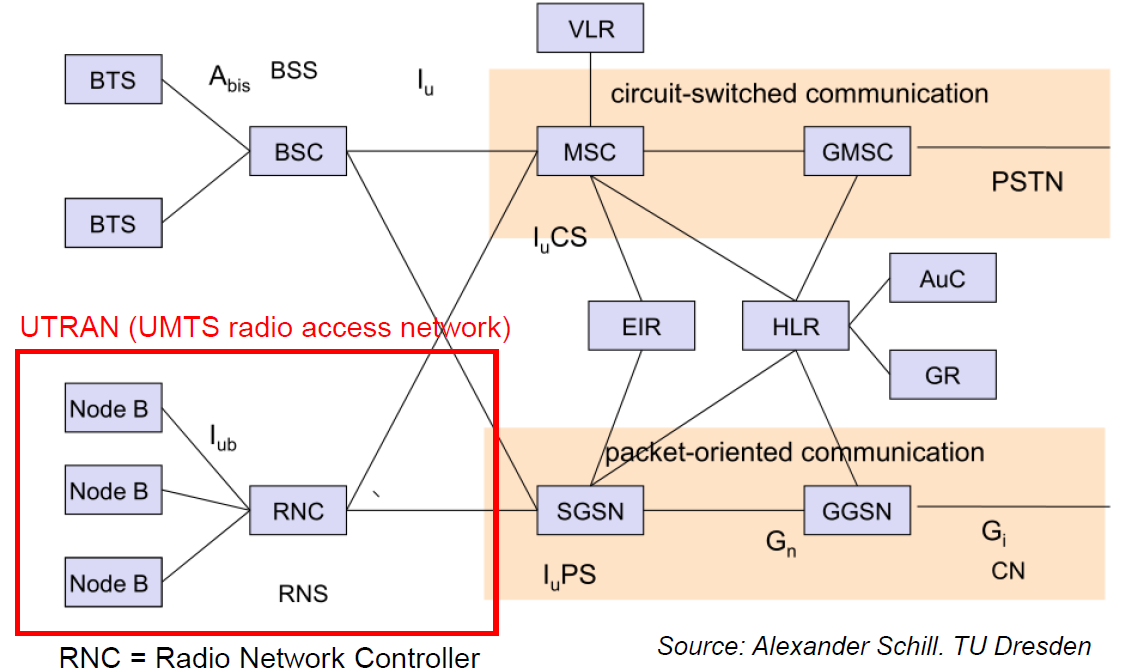
\includegraphics[scale=0.5]{img/umts.png}
\end{center}

\subsection{UMTS radio interface}
GPRS is too slow for modern traffic, there is a high latency (up to 700ms) 
because the MS has to request access to PDTCH.
\begin{itemize}
    \item UMTS used \textbf{FDMA} with a few carrier frequencies with several MHz bandwith
        + \textbf{CDMA}

        \paragraph{CDMA}
        CDMA with code length $n$ encodes a data symbole in $n$ chips
        \begin{itemize}
            \item Ex: 1 with code 010011 $\to$ (-1 +1 -1 -1 +1 +1 )
            \item Systems that use CDMA have constant chip rate (determined by hardware),
                UMTS: 3.84 MChips/s
        \end{itemize}

        \begin{tabular}{lm{10cm}}
            Using long code: &
            \begin{itemize}
                    \proitem{} Many senders can send simultaneously
                    \proitem{} Transmission errors can be detected easily
                    \consitem{} Data rate is slow with constant chip rate
            \end{itemize}
        \end{tabular}

    \item With CDMA, all User Equipment (=MS) can send simultaneously but to save
        bandwidth, the BS assigns a longer CDMA code to an idle UE:
        \begin{itemize}
            \item Longer code $\to$ more chips on the radio interface needed
                $\to$ lower effective transmission rate
            \item When the UE becomes active, it is slow at beginning but it can still
                send/receive data immediately 
            \item Same for UE that send low-bandwidth traffic, e.g voice
        \end{itemize}
\end{itemize}

\subsection{Cell planning}
With CDMA, many MS can use same frequency but the BS only uses one frequency.
This make planning frequencies for cells much easier since neighbor cells can use
same frequency but it require good transmission power control:
\begin{itemize}
	\item CDMA requires that the base station receives the signals 
	of all MSs with more or less same power
	\begin{itemize}
		\item BS can send power control instructions to MS up to
		1500 times per second
	\end{itemize}
	\item When adding a new cell: decrease transmission power of neighbor cells
\end{itemize}

\subsection{Channels}
UMTS defines different signaling and data channels
\begin{itemize}
	\item Logical channels
	\item Transport channels: between logical and physical channels.
	Prepare data frames for physical channels
	\item Physical channels
\end{itemize}

\subsection{Radio Access Bearer (RAB)}
UMTS is used for many different kinds of services: voices, video streaming, \ldots
\begin{itemize}
    \item The UE does not request a channel but a Bearer with certain QoS properties:
        \begin{itemize}
            \item Maximum speed
            \item Guaranteed speed
            \item Delay
            \item Error probability
            \item Type of traffic (voice,streaming,\ldots)
        \end{itemize}
    \item The UMTS network is responsible for establishing a connection that fits the 
        description
\end{itemize}

\subsection{Handover}
\begin{itemize}
    \item \textbf{Hard Handover}
        \begin{itemize}
            \item Similar to handover in GSM
            \item Takes around 100ms
        \end{itemize}

    \item \textbf{Soft Handover}: Data streams not only sent to/received
        from current cell, but also to/from up to 6 neighbor cells.\\
        Handover decision can be made for each frame

        \begin{itemize}
                \proitem{} Smooth handover with very small delay
                \proitem{} MS and BS can reduce transmission power
                \begin{itemize}
                    \item In GSM, MS would increase transmission power in a bad cell
                        until handover is unavoidable
                    \item In UMTS, MS works in several cells at the same time, 
                        compensating for the decreased quality of one cell
                \end{itemize}
                \consitem{} Requires more processing power in MS
                \consitem{} the traffic is duplicated $\Rightarrow$ Cell
                planning so that not more then 3 cells needed for soft
                handover.
        \end{itemize}
\end{itemize}

\subsection{Security}
\begin{itemize}
    \item \textbf{Authentication}:
        Authentication Center generates an authentication token that is checked by the 
        MS $\to$ network is authenticated.
    \item \textbf{Encryption of calls/data}
        Encryption is done between MS and RNC with 128-bits keys. 

        New algorithms are used instead of Ax
\end{itemize}

\subsection{HSPA and HSPA+}
\begin{itemize}
    \item \textbf{High-Speed Packet Access} is an extension for UMTS
        \begin{itemize}
            \item Up to 14.4 Mbit/s
            \item TDMA channel bundling
            \item Improved coding
            \item Latency = 100ms
        \end{itemize}

    \item \textbf{HSPA+}
        \begin{itemize}
            \item Up to 28 Mbit/s
            \item Improved coding
            \item MIMO(Multiple Input-Multiple Output)
                \begin{itemize}
                    \item Multiple antennas on sender and receiver side
                    \item Increased data rate and transmission quality
                \end{itemize}
                \begin{center}
                    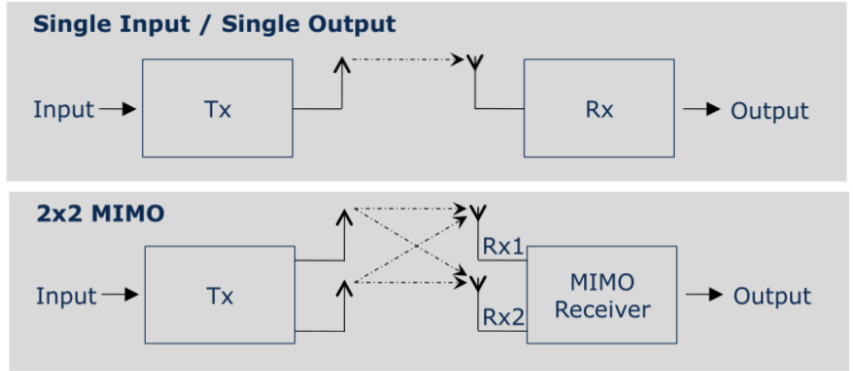
\includegraphics[width=0.7\linewidth]{img/mimo.png}
                \end{center}
        \end{itemize}
\end{itemize}

